\documentclass[11pt, twocolumn]{article}

\usepackage[margin=0.75in]{geometry}
\usepackage{graphicx}
\usepackage{amsmath, amssymb}
\usepackage{booktabs}
\usepackage{hyperref}
\usepackage{enumitem}
\usepackage{xcolor}
\usepackage{float}
\usepackage{caption}
\usepackage{subcaption}
\usepackage{titlesec}
\usepackage{tikz}
\usetikzlibrary{positioning, arrows.meta, fit, backgrounds}

\graphicspath{{assets/results/}}

\titlespacing*{\section}{0pt}{10pt}{5pt}
\titlespacing*{\subsection}{0pt}{8pt}{4pt}
\titlespacing*{\subsubsection}{0pt}{6pt}{3pt}

\setlength{\parskip}{4pt}
\setlength{\parindent}{0pt}

\title{
\textbf{Construction Site Safety Intelligence Dashboard} \\[6pt]
\large An ML-Powered End-of-Shift Safety Reporting System \\
Using Multi-Stage Vision Pipelines and Adversarial VLM Verification \\[6pt]
\normalsize UMD IronSite Hackathon 2026
}

\author{
Neel Mokaria \and Rajveer Singh \and Ananth Sriram \\[4pt]
\normalsize University of Maryland, College Park \\
\normalsize \texttt{\{nmokaria, rajveer, asriram2\}@terpmail.umd.edu}
}

\date{February 2026}

\begin{document}
\maketitle

% ----------------------------------------------------------------
\begin{abstract}
Construction remains the deadliest industry sector in the United States, with approximately 1,075 fatal worker injuries recorded in 2023 alone. The majority of these incidents are preventable, yet no affordable, passive, continuous monitoring system exists that can observe multiple workers across a site, maintain persistent identities, and produce actionable OSHA-aligned safety reports without real-time human review. We present the \textbf{Construction Site Safety Intelligence Dashboard}, an ML-powered end-of-shift reporting system that processes video from two independent camera modalities---POV body-worn and fixed wall-mounted cameras---through a unified three-stage pipeline: (1) fine-tuned YOLO for primary detection, (2) SAM~3 for segmentation refinement and worker deduplication, and (3) fine-tuned Qwen3-VL-8B-Instruct with a novel three-pass adversarial chain-of-thought protocol for compliance verification and hallucination control. The system detects PPE violations, ergonomic/musculoskeletal risks via REBA-inspired pose analysis, proximity hazards, and behavioral violations, mapping all findings to specific OSHA standards. A Next.js dashboard aggregates results into per-worker safety reports with timestamped evidence, violation logs, and compliance summaries.
\end{abstract}

% ----------------------------------------------------------------
\section{Introduction}

The Bureau of Labor Statistics reported a fatal work injury rate of 9.6 deaths per 100,000 full-time equivalent workers in the U.S. construction sector in 2023, making it the industry with the most fatalities of any sector~\cite{bls2023}. Men accounted for 91.5\% of fatalities. Fall protection (OSHA Standard 1926.501) alone accounts for the single largest violation category cited by OSHA year over year~\cite{osha2024}.

The core gap is operational: no affordable, passive, continuous monitoring system exists that can watch multiple workers across a construction site, resolve their identities over time, and produce an actionable report without requiring real-time human review. Existing solutions are either prohibitively expensive, require dedicated real-time operators, or cover only a narrow slice of the problem---for instance, hard hat detection alone.

We address this gap with an \textit{end-of-shift} processing paradigm. Rather than streaming video in real time, our system processes footage after a shift completes, making it practical to deploy on commodity hardware while using higher-quality models (including an 8-billion-parameter vision-language model) and multi-pass verification that would be infeasible under real-time latency constraints.

Our contributions are as follows:
\begin{enumerate}[nosep, leftmargin=*]
    \item A unified three-stage pipeline (YOLO $\rightarrow$ SAM~3 $\rightarrow$ VLM) that handles both PPE and posture/ergonomic analysis from two independent camera modalities.
    \item A three-pass adversarial chain-of-thought VLM protocol that significantly reduces hallucinated violations compared to single-pass prompting.
    \item REBA-inspired ergonomic risk scoring from YOLO pose keypoints with tuned confidence gates.
    \item A full-stack deployment with a Next.js dashboard, FastAPI backend, and SQLite persistence layer producing OSHA-mapped per-worker safety reports.
\end{enumerate}

% ----------------------------------------------------------------
\section{Related Work}

PPE detection on construction sites has been studied extensively using object detection models. Fang et al.~\cite{fang2018} applied Faster R-CNN to hard hat detection from surveillance footage. More recent work by Nath et al.~\cite{nath2020} used YOLOv3 for multi-class PPE detection. However, most existing systems address a single PPE category (typically hard hats) from a single camera viewpoint and do not maintain worker identity across frames.

Ergonomic risk assessment in construction has traditionally relied on manual observation methods such as REBA (Rapid Entire Body Assessment)~\cite{hignett2000} and RULA (Rapid Upper Limb Assessment). Recent computer vision approaches have attempted to automate these assessments using pose estimation~\cite{yan2017}, but few integrate pose-based ergonomic analysis into a unified pipeline alongside PPE detection.

Vision-language models (VLMs) have shown promise for visual understanding tasks, but their application to safety-critical domains raises concerns about hallucination---the generation of plausible but factually incorrect outputs. Our adversarial multi-pass approach draws conceptual inspiration from adversarial learning and self-consistency techniques~\cite{wang2022} adapted to the VLM verification setting.

The Segment Anything Model (SAM)~\cite{kirillov2023} and its successors have demonstrated strong zero-shot segmentation capabilities. We leverage SAM~3 not for standalone segmentation but as a refinement layer that improves bounding box precision and enables reliable PPE-to-worker association.

% ----------------------------------------------------------------
\section{System Architecture}

Both the posture/ergonomics stream and PPE violation detection stream share a common three-stage architecture. Artifacts flow sequentially, with the VLM consuming refined outputs from Stages~1--2 plus raw video or key frames. Figure~\ref{fig:pipeline} illustrates the end-to-end flow.

\begin{figure*}[t]
\centering
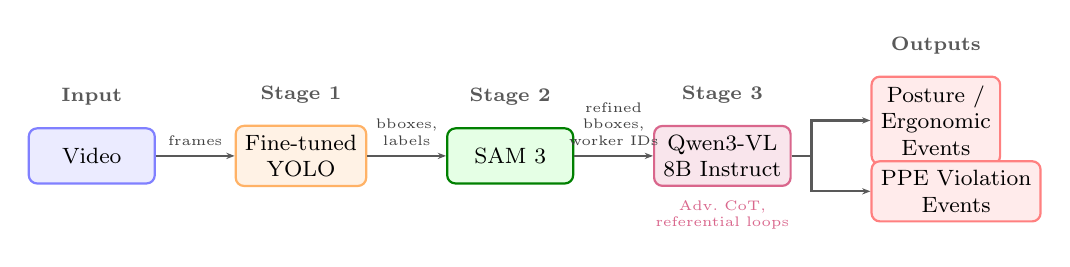
\begin{tikzpicture}[
    node distance=0.4cm and 0.6cm,
    >={Stealth[length=3pt]},
    stage/.style={draw, rounded corners=3pt, minimum height=0.7cm, minimum width=1.6cm, font=\footnotesize, align=center, thick},
    input/.style={stage, fill=blue!8, draw=blue!50},
    s1/.style={stage, fill=orange!10, draw=orange!60},
    s2/.style={stage, fill=green!10, draw=green!50!black},
    s3/.style={stage, fill=purple!10, draw=purple!60},
    outstyle/.style={stage, fill=red!8, draw=red!50},
    grplabel/.style={font=\scriptsize\bfseries, text=gray!70!black},
    arr/.style={->, thick, gray!70!black},
    arrlabel/.style={font=\tiny, text=gray!50!black, midway},
]
% Input
\node[input] (vid) {Video};

% Stage 1
\node[s1, right=1.0cm of vid] (yolo) {Fine-tuned\\YOLO};

% Stage 2
\node[s2, right=1.0cm of yolo] (sam) {SAM~3};

% Stage 3
\node[s3, right=1.0cm of sam] (vlm) {Qwen3-VL\\8B Instruct};

% Outputs
\node[outstyle, right=1.0cm of vlm, yshift=0.45cm] (pos) {Posture /\\Ergonomic\\Events};
\node[outstyle, right=1.0cm of vlm, yshift=-0.45cm] (ppe) {PPE Violation\\Events};

% Group labels
\node[grplabel, above=0.15cm of vid] {Input};
\node[grplabel, above=0.15cm of yolo] {Stage 1};
\node[grplabel, above=0.15cm of sam] {Stage 2};
\node[grplabel, above=0.15cm of vlm] {Stage 3};
\node[grplabel, above=0.15cm of pos] {Outputs};

% Arrows
\draw[arr] (vid) -- node[arrlabel, above] {frames} (yolo);
\draw[arr] (yolo) -- node[arrlabel, above, text width=1.2cm, align=center] {bboxes,\\labels} (sam);
\draw[arr] (sam) -- node[arrlabel, above, text width=1.4cm, align=center] {refined bboxes,\\worker IDs} (vlm);
\draw[arr] (vlm.east) -- ++(0.25,0) |- (pos.west);
\draw[arr] (vlm.east) -- ++(0.25,0) |- (ppe.west);

% Method label under VLM
\node[font=\tiny, text=purple!60, below=0.05cm of vlm, text width=1.8cm, align=center] {Adv.\ CoT,\\referential loops};

\end{tikzpicture}
\caption{Three-stage pipeline architecture shared by both posture/ergonomics and PPE violation detection. Video frames pass through YOLO detection, SAM~3 refinement, and adversarial VLM verification to produce compliance-checked safety events.}
\label{fig:pipeline}
\end{figure*}

\begin{table*}[t]
\centering
\small
\caption{Three-stage pipeline: components, roles, and outputs.}
\label{tab:pipeline}
\begin{tabular}{cl p{5.2cm} p{4.8cm}}
\toprule
\textbf{Stage} & \textbf{Component} & \textbf{Role} & \textbf{Output} \\
\midrule
1 & Fine-tuned YOLO & First pass on video: detect workers, PPE items, poor-posture candidates, violation candidates & Initial bounding boxes, class labels, frame-level detections \\[3pt]
2 & SAM~3 & Worker tagging, deduplication, refined masks and bboxes (MoE segmentation) & Refined bboxes, worker/track IDs, segmentation masks \\[3pt]
3 & Qwen3-VL-8B-Instruct & Validates Stage 1--2 outputs via method prompting, chain-of-thought, and referential loops; enforces OSHA; reduces hallucination & Compliance-checked violation flags $\rightarrow$ final posture/ergonomic and PPE violation outputs \\
\bottomrule
\end{tabular}
\end{table*}

\subsection{Stage 1: Primary Detection (Fine-tuned YOLO)}

We fine-tuned YOLO11 on a composite dataset assembled from multiple construction-specific PPE sources: Ultralytics Construction-PPE (11 classes), Roboflow construction site safety, SH17, and additional PPE datasets from Kaggle. The detector recognizes 12 mapped classes:

\begin{table}[H]
\centering
\small
\caption{YOLO class mapping for wall-cam detection.}
\begin{tabular}{ll}
\toprule
\textbf{Raw Class} & \textbf{Mapped Label} \\
\midrule
person & worker \\
helmet / no helmet & hardhat / no\_hardhat \\
vest / no vest & safety\_vest / no\_safety\_vest \\
gloves / no gloves & gloves / no\_gloves \\
excavator, truck & excavator, dump\_truck \\
crane, forklift & crane, forklift \\
ladder, scaffold & ladder, scaffold \\
\bottomrule
\end{tabular}
\end{table}

For wall-cam footage, we run YOLO with \textbf{BoT-SORT} tracking to maintain persistent track IDs across frames, enabling temporal PPE accumulation per worker.

For posture analysis, a separate YOLO pose model extracts 17 COCO keypoints per detected person, providing the joint coordinates needed for ergonomic angle computation.

The detection confidence threshold is set deliberately low at $\tau_{\text{conf}} = 0.15$ to maximize recall; false positives are handled downstream by the VLM verification stage.

\subsection{Stage 2: Refinement and Deduplication (SAM~3)}

YOLO bounding boxes are passed to SAM~3 (Segment Anything Model~3) as box prompts to generate pixel-accurate segmentation masks. This stage serves three purposes:

\begin{enumerate}[nosep, leftmargin=*]
    \item \textbf{Bounding box refinement}: SAM~3 masks tighten noisy YOLO boxes, improving the visual evidence quality of annotated frames.
    \item \textbf{Worker-level segmentation}: Per-worker masks provide clean crops for VLM input and dashboard display.
    \item \textbf{PPE-to-worker association}: For each detected PPE item, we check which worker's bounding box contains the item's center point. This center-point containment logic resolves ambiguity when workers are clustered together.
\end{enumerate}

Worker safety logs accumulate PPE detections over time. Required PPE is defined as $\mathcal{P}_{\text{req}} = \{\text{hardhat}, \text{safety\_vest}, \text{gloves}\}$. If a tracked worker has not been observed with a required item after sufficient frames, the system flags a violation.

\subsection{Stage 3: Compliance Verification (Qwen3-VL-8B-Instruct)}

The VLM stage is designed to address the critical problem of hallucination in safety-critical applications. We employ a \textbf{three-pass adversarial chain-of-thought} protocol:

\textbf{Pass 1---Generator (``Jamie Reyes''):} A field safety inspector persona with 6 years of on-site experience reviews raw video only, with no access to machine detection data. The model produces free-form inspection notes, providing an independent observational signal.

\textbf{Pass 2---Discriminator (``Marcus Chen''):} A Chief Safety Officer persona with 24 years of experience independently reviews the video alongside YOLO/SAM annotated frames (bounding boxes and masks overlaid). This pass has no access to Pass~1 notes and validates machine detections from an independent perspective.

\textbf{Pass 3---Reconciler (``Marcus Chen''):} The same CSO persona reconciles all three information sources---Jamie's notes, Marcus's independent assessment, and raw YOLO/SAM data---into a structured JSON assessment containing hazard types, severity levels, explanations, and recommendations.

\subsubsection{Confidence Calibration}

The VLM receives YOLO confidence scores as calibration signals:

\begin{table}[H]
\centering
\small
\caption{Confidence calibration bands for VLM priors.}
\begin{tabular}{lll}
\toprule
\textbf{YOLO Conf.} & \textbf{Signal} & \textbf{VLM Guidance} \\
\midrule
$\geq 0.70$ & HIGH & Strong prior: detection is real \\
$0.40$--$0.69$ & MODERATE & Verify visually \\
$0.15$--$0.39$ & WEAK & Must confirm in video \\
$< 0.15$ & NOISE & Discard unless confirmed \\
\bottomrule
\end{tabular}
\end{table}

The VLM was optionally fine-tuned with a LoRA adapter for construction-specific understanding. Long videos are chunked into 60-second segments to prevent context window overflow; each chunk receives an independent VLM assessment.

The final VLM output is a structured \texttt{VLMAssessment} object containing: scene summary, worker count, equipment present, per-worker PPE status (each item marked \texttt{PRESENT}/\texttt{ABSENT}/\texttt{UNCLEAR}), a list of typed hazards with severity and explanation, overall confidence, and actionable recommendations.

% ----------------------------------------------------------------
\section{Posture and Ergonomic Analysis}

For POV body-worn camera footage, we implement a REBA-inspired ergonomic risk assessment pipeline.

\subsection{Joint Angle Extraction}

From the 17 COCO keypoints produced by the YOLO pose model, we compute six ergonomic angles:

\begin{itemize}[nosep, leftmargin=*]
    \item \textbf{Trunk flexion} ($\theta_{\text{trunk}}$): Forward lean of the spine, computed from the midpoint of hip-to-shoulder vectors relative to vertical.
    \item \textbf{Trunk lateral lean} ($\theta_{\text{lat}}$): Sideways deviation of the trunk.
    \item \textbf{Neck flexion} ($\theta_{\text{neck}}$): Head position relative to the trunk midline.
    \item \textbf{Knee angle} ($\theta_{\text{knee}}$): Degree of squat or kneeling.
    \item \textbf{Arm raise} ($\theta_{\text{arm}}$): Maximum elevation of either arm above shoulder level.
    \item \textbf{Elbow flexion} ($\theta_{\text{elbow}}$): Degree of arm bend.
\end{itemize}

\subsection{REBA-Inspired Risk Scoring}

Joint angles are combined into a risk score using a two-group scheme inspired by the Rapid Entire Body Assessment (REBA) method~\cite{hignett2000}:

\begin{align}
\text{Score}_A &= f(\theta_{\text{trunk}}, \theta_{\text{neck}}, \theta_{\text{knee}}, \theta_{\text{lat}}) \\
\text{Score}_B &= g(\theta_{\text{arm}}, \theta_{\text{elbow}}) \\
\text{Combined} &= \max(\text{Score}_A, \text{Score}_B) + \Delta
\end{align}

where $\Delta$ captures interaction effects (e.g., simultaneous trunk twist and arm raise).

\subsection{Violation Classification}

The combined score maps to violation types with tuned thresholds:

\begin{table}[H]
\centering
\small
\caption{Posture violation classification thresholds.}
\begin{tabular}{lll}
\toprule
\textbf{Condition} & \textbf{Type} & \textbf{Risk} \\
\midrule
Combined $< 3$ & Compliant & Level 1 \\
Combined $\geq 3$ & \texttt{AWKWARD\_POSTURE} & Level 2 \\
Combined $\geq 5$ & \texttt{OVERREACH} & Level 3 \\
Combined $\geq 8$ & \texttt{MSD\_HIGH\_RISK} & Level 4 \\
\bottomrule
\end{tabular}
\end{table}

Specific violation triggers include:
\begin{itemize}[nosep, leftmargin=*]
    \item \texttt{OVERREACH}: Arm elevation $> 65^\circ$ with concurrent body twist.
    \item \texttt{AWKWARD\_POSTURE}: Trunk flexion $> 48^\circ$ without load context.
    \item \texttt{MSD\_HIGH\_RISK}: Trunk flexion $> 65^\circ$ at risk level 4.
    \item \texttt{KNEELING\_SQUATTING\_LOW}: Deep knee bend with forward lean.
\end{itemize}

A minimum keypoint confidence gate of $\tau_{\text{kp}} = 0.65$ is enforced to prevent false positives from poorly-detected poses. The ``trunk good max'' threshold is set at $38^\circ$ based on iterative tuning against our annotated test datasets.

% ----------------------------------------------------------------
\section{Worker Identity and Object Permanence}

Maintaining consistent worker identity across an entire shift is a core technical challenge, particularly for the wall-cam system where workers move in and out of frame and get occluded.

\textbf{Tracking:} BoT-SORT integrated with YOLO provides frame-to-frame track continuity, handling short-term occlusions.

\textbf{Identity Database:} Each worker is stored with a persistent UUID, site association, and optional appearance embedding (base64-encoded). The database persists across days, allowing violation history to accumulate.

\textbf{Object Permanence:} When a tracked worker disappears from frame, the system holds their last known state (ID, embedding, position) in memory. On reappearance, the system performs embedding similarity matching to re-associate the worker with their existing ID rather than creating a duplicate.

\textbf{PPE Temporal Accumulation:} Per-worker safety logs track which PPE items have been observed over time. This temporal smoothing prevents momentary detection failures from triggering false violations.

% ----------------------------------------------------------------
\section{OSHA Violation Coverage}

The system maps detected violations to specific OSHA standards. Table~\ref{tab:osha} summarizes the coverage by camera modality.

\begin{table}[H]
\centering
\small
\caption{OSHA violation coverage by detection modality.}
\label{tab:osha}
\begin{tabular}{lll}
\toprule
\textbf{Standard} & \textbf{Violation} & \textbf{Source} \\
\midrule
1926.501 & Fall protection & Wall cam \\
1926.503 & Training compliance & Worker DB \\
1926.451 & Scaffolding violations & Wall cam \\
1926.102 & Eye/face PPE & Wall cam \\
1910.212 & Machine guarding & Wall cam \\
Ergonomic & MSD risk, posture & POV \\
Ladder & Improper use & Wall cam \\
Respiratory & Missing respirator & Wall cam \\
\bottomrule
\end{tabular}
\end{table}

Violations are scored by severity (\texttt{LOW}, \texttt{MEDIUM}, \texttt{HIGH}, \texttt{CRITICAL}) and frequency. Workers with repeated violations are surfaced prominently in the dashboard report.

% ----------------------------------------------------------------
\section{System Implementation}

\subsection{Backend}

The backend is implemented as a FastAPI application with async job processing. Key implementation details:

\begin{itemize}[nosep, leftmargin=*]
    \item \textbf{Model pre-warming:} All models (YOLO, SAM~3, Qwen3-VL) are loaded on startup in a thread pool executor to avoid cold-start OOM errors.
    \item \textbf{Job pipeline:} Video processing runs as background tasks with progress tracking (0--100\%) and stage reporting.
    \item \textbf{Event deduplication:} Safety events are deduplicated per (worker, violation type) per shift to prevent over-counting from multi-frame detections.
    \item \textbf{Database:} SQLite via SQLAlchemy with four core tables---\texttt{sites}, \texttt{workers}, \texttt{shifts}, and \texttt{safety\_events}---plus denormalized counters on workers and shifts for dashboard performance.
\end{itemize}

The wall-cam pipeline (\texttt{wall\_cam.py}) processes every 3rd frame, running YOLO with BoT-SORT, SAM~3 mask generation, PPE association, and proximity hazard detection (worker-to-equipment distance normalized by frame diagonal, threshold $d_{\text{prox}} = 0.25$). The posture pipeline (\texttt{posture.py}) runs concurrently in a thread pool.

\subsection{Frontend Dashboard}

The dashboard is built with Next.js~14 and TypeScript, communicating with the backend via a typed API client. Key views include:

\begin{itemize}[nosep, leftmargin=*]
    \item \textbf{Dashboard home:} KPIs (jobs processed, violations detected, total events), backend status indicator, recent jobs.
    \item \textbf{Job detail:} Live progress bar, posture analysis summary, hazard breakdown, per-worker PPE compliance cards, expandable violation log with annotated frame evidence.
    \item \textbf{Ingest:} Drag-and-drop video upload for POV or wall-cam modes, with live job status polling at 2-second intervals.
\end{itemize}

\subsection{Infrastructure}

The system was developed and tested on 4$\times$ NVIDIA RTX PRO 6000 Blackwell GPUs. Video chunks of 60 seconds keep VLM context within bounds. Frame sampling at every 3rd frame balances detection coverage with processing throughput.

% ----------------------------------------------------------------
\section{Data and Datasets}

We assembled training and validation data from multiple sources:

\textbf{PPE detection training:} Ultralytics Construction-PPE (11 classes), Roboflow construction site safety, SH17, and additional PPE datasets---used to fine-tune the YOLO11 detector.

\textbf{Posture reference:} The CWPV (Construction Working Postures Videos) dataset from Figshare, containing POV footage of construction workers annotated for musculoskeletal posture analysis.

\textbf{Behavioral reference:} \"Onal \& Dand{\i}l video dataset (691 clips, 8 behaviour classes) from fixed IP cameras, used as reference for wall-cam behavioural classification.

\textbf{Validation:} Long-form POV videos (15--20+ minutes per clip) from construction scenarios (masonry, prep, transit). We exported compliant and non-compliant clips into \texttt{Testing\_Data\_Posture} and \texttt{Testing\_Data\_PPE} directories for threshold tuning and human review. Frame-level exports (every 8 frames) supported agreement analysis.

% ----------------------------------------------------------------
\section{Results and Discussion}

The pipeline was validated on multiple hours of construction site footage across both camera modalities. Figures~\ref{fig:ppe} and~\ref{fig:posture} show representative outputs.

\textbf{PPE detection:} The system correctly identifies hard hats, safety vests, and gloves on compliant workers, and flags missing PPE with bounding box evidence. Figure~\ref{fig:ppe} shows a compliant detection (safety vest identified, green label) alongside a violation (missing glove flagged with red bounding box). The wall-cam pipeline detects violations from site-wide views, while POV cameras capture hand-level PPE such as gloves.

\begin{figure}[H]
\centering
\begin{subfigure}[t]{0.48\columnwidth}
    
\includegraphics[width=\linewidth]{ppe_compliant.png}
    \caption{Compliant: safety vest detected.}
\end{subfigure}
\hfill
\begin{subfigure}[t]{0.48\columnwidth}
    
\includegraphics[width=\linewidth]{ppe_violation.png}
    \caption{Violation: no glove flagged.}
\end{subfigure}
\caption{PPE detection results. (a)~Worker building a concrete block wall; system identifies the high-visibility vest and labels the worker as compliant. (b)~POV frame; system flags an exposed hand with a red bounding box for missing hand protection.}
\label{fig:ppe}
\end{figure}

\textbf{Posture analysis:} The REBA-inspired scoring successfully distinguishes between compliant postures (e.g., upright standing, normal tool handling) and at-risk postures (e.g., overreach classified at risk level~3, deep trunk flexion classified as MSD high risk). Figure~\ref{fig:posture} contrasts a compliant posture assessment with an overreach violation. The confidence gate at $\tau_{\text{kp}} = 0.65$ effectively filters spurious detections from partial occlusions.

\begin{figure}[H]
\centering
\begin{subfigure}[t]{0.48\columnwidth}
    
\includegraphics[width=\linewidth]{posture_good.png}
    \caption{Worker \#825: Posture Good.}
\end{subfigure}
\hfill
\begin{subfigure}[t]{0.48\columnwidth}
    
\includegraphics[width=\linewidth]{posture_risk_overreach.png}
    \caption{Worker \#910: Risk 3 --- Overreach.}
\end{subfigure}
\caption{Posture analysis results. (a)~Worker segmented with blue mask and green bounding box; pose and PPE assessed as compliant. (b)~Worker segmented with red box; elevated arm classified as OVERREACH with risk level~3 for musculoskeletal strain.}
\label{fig:posture}
\end{figure}

\textbf{VLM verification:} The three-pass adversarial protocol reduces hallucinated violations compared to single-pass prompting. The reconciliation pass (Pass~3) resolves conflicts between the generator and discriminator, producing structured assessments with calibrated confidence levels.

\subsection{Limitations}

Several limitations remain:

\begin{itemize}[nosep, leftmargin=*]
    \item \textbf{Re-ID accuracy:} Worker re-identification in dense, crowded scenes has not been fully stress-tested. The embedding matching infrastructure is designed but requires validation at scale.
    \item \textbf{PPE false positives:} Variable lighting conditions cause intermittent false positive PPE detections.
    \item \textbf{Posture thresholds:} The boundary between ``safe'' and ``borderline'' posture remains sensitive to threshold choices and may need per-site calibration.
    \item \textbf{POV occlusion:} Body-worn cameras frequently experience view obstruction mid-task, limiting the signal available for posture and PPE analysis.
\end{itemize}

% ----------------------------------------------------------------
\section{Challenges}

\textbf{VLM hallucination} was the single largest technical obstacle. Early single-pass VLM runs would confidently report nonexistent violations. The adversarial multi-pass architecture---where two independent ``inspector'' personas assess the same scene before a reconciliation pass---was the key design that brought hallucination rates to acceptable levels.

\textbf{PPE-to-worker association} is nontrivial when workers cluster together. A hard hat detection floating above a worker's bounding box does not automatically belong to that worker. Center-point containment logic combined with temporal smoothing across frames was required for reliable association.

\textbf{Ergonomic threshold tuning} required extensive iteration against annotated test clips. The distinction between normal construction activity and hazardous posture is inherently ambiguous---a $45^\circ$ trunk lean may be safe for a momentary tool pickup but dangerous if sustained.

\textbf{GPU memory management} across three large models (YOLO, SAM~3, 8B-parameter VLM) demanded careful orchestration: pre-warming on startup, sequential inference staging, and 60-second video chunking to prevent OOM failures.

% ----------------------------------------------------------------
\section{Future Work}

\begin{itemize}[nosep, leftmargin=*]
    \item \textbf{Full re-ID deployment:} Stress-testing appearance embedding matching in dense multi-worker footage to enable robust violation history tracking.
    \item \textbf{Real-time streaming:} Adding RTSP/WebRTC ingestion for live monitoring with periodic batch VLM verification.
    \item \textbf{Site heatmaps:} Aggregating per-frame worker positions into occupancy heatmaps overlaid on site floorplans.
    \item \textbf{Expanded OSHA taxonomy:} Adding detection for electrical, trenching, and hazard communication violations.
    \item \textbf{EHS platform integration:} Exporting reports to Procore, Autodesk Construction Cloud, and standard EHS formats.
    \item \textbf{Site-specific fine-tuning:} Calibration workflows where a site uploads footage and the system auto-tunes detection thresholds for local conditions.
\end{itemize}

% ----------------------------------------------------------------
\section{Conclusion}

We have presented the Construction Site Safety Intelligence Dashboard, an end-of-shift ML pipeline that processes construction site video through three stages---YOLO detection, SAM~3 refinement, and adversarial VLM verification---to produce OSHA-aligned per-worker safety reports. The system handles two camera modalities (POV and wall-mounted) through a unified architecture, performs REBA-inspired ergonomic risk scoring from pose estimation, and employs a novel three-pass adversarial chain-of-thought protocol to control VLM hallucination in safety-critical assessments. The accompanying Next.js dashboard provides an accessible interface for site supervisors to review violations with frame-level evidence. While limitations remain in re-identification robustness and threshold sensitivity, the system demonstrates that affordable, passive, end-of-shift safety monitoring is achievable with current vision and language models.

% ----------------------------------------------------------------
\begin{thebibliography}{10}
\small
\setlength{\itemsep}{1pt}
\setlength{\parskip}{0pt}

\bibitem{bls2023}
Bureau of Labor Statistics. \textit{Census of Fatal Occupational Injuries Summary, 2023}. U.S. Department of Labor, 2024.

\bibitem{osha2024}
Occupational Safety and Health Administration. \textit{Top 10 Most Frequently Cited Standards for Fiscal Year 2024}. U.S. Department of Labor, 2024. \url{https://www.osha.gov/top10citedstandards/}

\bibitem{fang2018}
Q.~Fang, H.~Li, X.~Luo, L.~Ding, H.~Luo, T.~Rose, and W.~An. Detecting non-hardhat-use by a deep learning method from far-field surveillance videos. \textit{Automation in Construction}, 85:1--9, 2018.

\bibitem{nath2020}
N.~D. Nath, A.~H. Behzadan, and S.~G. Paal. Deep learning for site safety: Real-time detection of personal protective equipment. \textit{Automation in Construction}, 112:103085, 2020.

\bibitem{hignett2000}
S.~Hignett and L.~McAtamney. Rapid Entire Body Assessment (REBA). \textit{Applied Ergonomics}, 31(2):201--205, 2000.

\bibitem{yan2017}
X.~Yan, H.~Li, A.~R. Li, and H.~Zhang. Wearable IMU-based real-time motion warning system for construction workers' musculoskeletal disorders prevention. \textit{Automation in Construction}, 74:2--11, 2017.

\bibitem{wang2022}
X.~Wang, J.~Wei, D.~Schuurmans, Q.~Le, E.~Chi, S.~Narang, A.~Chowdhery, and D.~Zhou. Self-consistency improves chain of thought reasoning in language models. In \textit{Proc. ICLR}, 2023.

\bibitem{kirillov2023}
A.~Kirillov, E.~Mintun, N.~Ravi, H.~Mao, C.~Rolland, L.~Gustafson, T.~Xiao, S.~Whitehead, A.~Berg, W.-Y. Lo, P.~Doll{\'a}r, and R.~Girshick. Segment Anything. In \textit{Proc. ICCV}, 2023.

\bibitem{onal2024}
O.~\"Onal and E.~Dand{\i}l. A video dataset for safe/unsafe worker behaviour classification in production environments. \textit{BMC Research Notes}, 17:234, 2024.

\bibitem{cwpv2024}
CWPV: A Working Postures of the Construction Working Postures Videos dataset. \textit{Figshare}, 2024. \url{https://figshare.com/articles/dataset/27907818}

\end{thebibliography}

\end{document}
